\documentclass[10pt]{article}
\usepackage[a4paper,margin=0.9cm,top=0.7cm,bottom=0.7cm,columnsep=0.45cm]{geometry}
\usepackage[utf8]{inputenc}
\usepackage[T1]{fontenc}
\usepackage{lmodern}
\usepackage{microtype}
\usepackage{multicol}
\usepackage{booktabs}
\usepackage{xcolor}
\usepackage{hyperref}
\usepackage{tikz}
\usepackage{pgfplots}
\pgfplotsset{compat=1.17}
\usetikzlibrary{positioning,arrows.meta,calc}

\definecolor{ucblue}{RGB}{0,51,102}
\definecolor{ftorange}{RGB}{204,85,0}
\definecolor{toolgray}{RGB}{110,110,110}
\hypersetup{colorlinks=true,urlcolor=ucblue,linkcolor=ucblue}
\setlength{\parindent}{0pt}
\setlength{\parskip}{1.5pt}
\pagestyle{empty}
\newcommand{\head}[1]{\textbf{\color{ucblue}#1}\hspace{0.4em}}
\newcommand{\pendiente}[1]{\textcolor{red}{[PENDIENTE: #1]}}
% Completar después de la corrida en Colab (ver README, "Cómo reproducir el Deliverable 4").
\newcommand{\VideoURL}{\pendiente{link del video}}
\newcommand{\HFURL}{\href{https://huggingface.co/vicentesonez/sql4business-planificador-qlora}{huggingface.co/vicentesonez/sql4business-planificador-qlora}}
\newcommand{\LOSSCSV}{../results/deliverable4/adapter/loss.csv}

\begin{document}

\begin{center}
{\Large\bfseries\color{ucblue} SQL4Business: Deliverable 4 --- fine-tuning del Planificador}\\[1pt]
{\small Generative Artificial Intelligence (580694), Universidad de Concepci\'on}\\[1pt]
{\small Aredhel Jim\'enez, Bryan Riquelme, Guido Salazar, Vicente So\~nez}\\[1pt]
{\small C\'odigo: \href{https://github.com/aredhel-jmze/Asistente-SQL-4-Business}{github.com/aredhel-jmze/Asistente-SQL-4-Business}
\quad$\vert$\quad Adaptador: \HFURL \quad$\vert$\quad Video: \VideoURL}
\end{center}

\vspace{-6pt}
\begin{center}
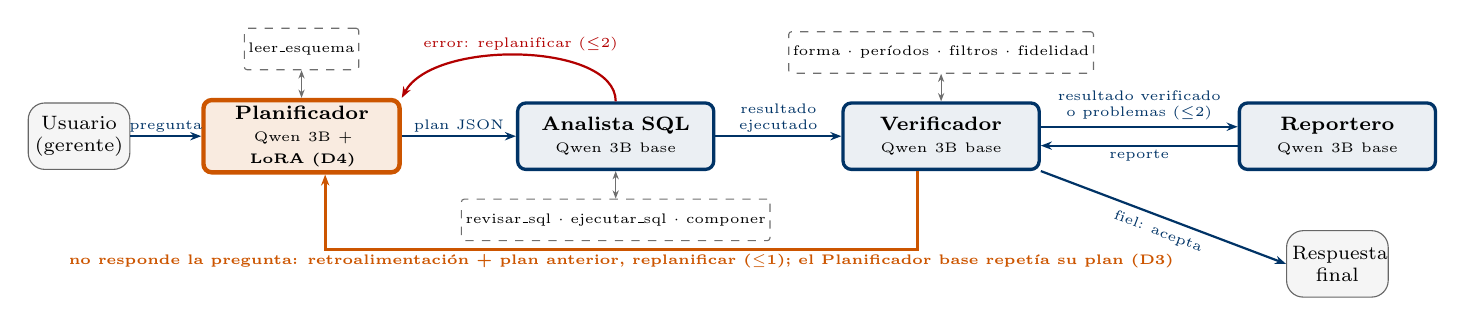
\begin{tikzpicture}[
  font=\scriptsize,
  agent/.style={draw=ucblue, fill=ucblue!8, very thick, rounded corners=3pt, align=center, minimum height=2.4em, text width=2.35cm, inner sep=2pt},
  ft/.style={agent, draw=ftorange, fill=ftorange!12, line width=1.6pt},
  tool/.style={draw=toolgray, dashed, rounded corners=1pt, align=center, font=\tiny, inner sep=1.5pt, minimum height=1.5em},
  ext/.style={draw=black!60, fill=black!4, rounded corners=6pt, align=center, minimum height=2.4em, text width=1.15cm, inner sep=2pt},
  flow/.style={-{Stealth[length=4pt]}, thick, ucblue},
  back/.style={-{Stealth[length=4pt]}, thick, red!70!black},
  use/.style={{Stealth[length=3pt]}-{Stealth[length=3pt]}, toolgray},
  lab/.style={font=\tiny, inner sep=1pt, align=center}]
  \node[ext] (u) {Usuario\\(gerente)};
  \node[ft, right=0.9cm of u] (p) {\textbf{Planificador}\\{\tiny Qwen 3B + \textbf{LoRA (D4)}}};
  \node[agent, right=1.45cm of p] (a) {\textbf{Analista SQL}\\{\tiny Qwen 3B base}};
  \node[agent, right=1.6cm of a] (v) {\textbf{Verificador}\\{\tiny Qwen 3B base}};
  \node[agent, right=2.5cm of v] (r) {\textbf{Reportero}\\{\tiny Qwen 3B base}};
  \node[ext, below=0.75cm of r] (o) {Respuesta\\final};
  \node[tool, above=0.35cm of p] (t1) {leer\_esquema};
  \node[tool, below=0.35cm of a] (t3) {revisar\_sql $\cdot$ ejecutar\_sql $\cdot$ componer};
  \node[tool, above=0.35cm of v] (t5) {forma $\cdot$ períodos $\cdot$ filtros $\cdot$ fidelidad};
  \draw[flow] (u) -- node[lab, above] {pregunta} (p);
  \draw[flow] (p) -- node[lab, above] {plan JSON} (a);
  \draw[flow] (a) -- node[lab, above] {resultado\\ejecutado} (v);
  \draw[flow] ($(v.east)+(0,0.12)$) -- node[lab, above=1pt] {resultado verificado\\o problemas ($\leq$2)} ($(r.west)+(0,0.12)$);
  \draw[flow] ($(r.west)+(0,-0.12)$) -- node[lab, below] {reporte} ($(v.east)+(0,-0.12)$);
  \draw[flow] (v.south east) -- node[lab, below=2pt, sloped] {fiel: acepta} (o.west);
  \draw[use] (t1) -- (p); \draw[use] (t3) -- (a); \draw[use] (t5) -- (v);
  \draw[back] (a.north) .. controls +(0,0.75) and +(0.4,0.75) .. node[lab, above] {error: replanificar ($\leq$2)} (p.north east);
  \draw[back, ftorange, line width=1.2pt] ($(v.south)+(-0.3,0)$) -- ++(0,-1.0) -| node[lab, pos=0.25, below, text=ftorange] {\textbf{no responde la pregunta: retroalimentación + plan anterior, replanificar ($\leq$1); el Planificador base repetía su plan (D3)}} ($(p.south)+(0.3,0)$);
\end{tikzpicture}
\end{center}
\vspace{-9pt}
{\tiny Naranja: el agente ajustado (adaptador LoRA sobre el mismo modelo base, cargado una vez; los otros tres agentes usan los pesos base) y el ciclo que debía corregir. Por el comentario al D3, el Verificador revisa el resultado antes de que el Reportero redacte y luego la fidelidad del reporte (antes revisaba todo al final). Prompts versionados en \texttt{prompts/}; el texto que lee el modelo no cambió.}

\vspace{-2pt}
\begin{multicols}{2}
\small

\head{Tarea, falla y continuidad.} La misma tarea (pregunta de negocio $\rightarrow$ consultas SQL
necesarias y reporte fiel), la misma falla diagnosticada en el D1 (planificar preguntas combinadas:
0/5 con prompting directo) y el mismo sistema de cuatro agentes del D3, con el Verificador antes del
Reportero (comentario al D3: las 27 trazas del D3 reproducen sin GPU los mismos planes y resultados con
este orden; (3), (4) y el control se evalúan con él), con el mismo modelo
(\texttt{Qwen2.5-Coder-3B-Instruct}, rev.\ \texttt{488639f}, NF4, greedy) y el mismo criterio de
evaluación (\textit{sql}, \textit{answer}, \textit{e2e}).

\head{Elección del agente: el Planificador.} En la corrida final del D3, las 4 preguntas que el
sistema falla (q04, q10, q12, q11-p) nacen en un plan del Planificador; el Analista, el Reportero y
el Verificador no originan ningún error. Además, en 4 de las 6 veces que el Verificador o el Analista
le devolvieron el plan con el motivo exacto (``growth\_pct needs the earlier period first'', ``the
question names `Alimentos'\,''), el Planificador devolvió \emph{el mismo SQL}. El D3 ya agotó la vía
del prompting: few-shot, descomposición, controles nuevos del Verificador y un ejemplo más en v2;
detectar funciona, corregir no. Con decodificación greedy, el sesgo por el orden en que la pregunta
nombra los meses domina el texto de la retroalimentación. Por eso la intervención es sobre los
pesos: enseñar con ejemplos (a)~a ordenar los períodos por tiempo y no por mención, y (b)~a
\emph{usar} la retroalimentación del Verificador. El control mide si los mismos datos, dados como
prompt, bastan.

\head{Datos.} 1.282 pares (entrada, salida) para el rol del Planificador
(\texttt{data/finetune/}, regenerables con \texttt{scripts/build\_planner\_data.py}, semilla 4).
\textit{Entrada}: el prompt exacto que lee el Planificador en ejecución (esquema enriquecido,
técnicas del D3, pregunta). \textit{Salida}: el plan JSON correcto. \textit{Fuente}: plantillas de
preguntas (86\,\% español, 14\,\% inglés; con y sin tildes) sobre \texttt{business.db}, en 8 familias
(valor, líder, ficha, listado, crecimiento, participación, comparación de líderes, filtro + ranking).
\textit{Etiquetado}: ningún modelo escribe salidas; cada plan lo construye el código a partir de los
parámetros de la tarea, se ejecuta con las herramientas del Analista y se compara con un valor de
referencia calculado en Python sobre las tablas (0 discrepancias; se descartan empates).
883 ejemplos de \emph{plan} (51\,\% de los de crecimiento nombran primero el período posterior, como
q12) y 399 de \emph{reparación}: plan equivocado (orden invertido, filtro de categoría omitido,
participación como crecimiento, dos valores con \texttt{direct}, crecimiento en vez de comparar
líderes, listado en vez del primero, mes corrido) + la retroalimentación que produce la propia
función del Verificador $\rightarrow$ plan correcto. \textit{Revisión}: ningún modelo genera
datos, así que no hay salidas generadas que revisar a mano; los 1.282 pares se verifican por ejecución.
\textit{Separación}: de 4.737 tareas candidatas se eliminaron 216 con la misma operación y
resultados que una pregunta de evaluación, 182 con algún paso numérico igual a un paso de
evaluación y 52 con similitud de 5-gramas $\geq 0{,}5$; la máxima similitud que queda es 0,19 (con
q15-p). Train/dev (1.155/127) se separan por cálculo; un test lo comprueba.

\head{Entrenamiento.} QLoRA (\texttt{scripts/train\_planner.py}, bucle propio en PyTorch + PEFT
0.22): base NF4 de 4 bits, LoRA $r{=}16$, $\alpha{=}32$, dropout 0,05 en
\texttt{q,k,v,o,gate,up,down\_proj}; AdamW, lr $2\cdot10^{-4}$, calentamiento 5\,\% + coseno,
2 épocas, lote efectivo 8 (lote 1 $\times$ 8 acumulaciones), 290 pasos, bf16,
gradient checkpointing, largo máx.\ 2.560 tokens (máx.\ real 2.243); 29,9\,M parámetros entrenables. La
pérdida es la entropía cruzada solo sobre los tokens del plan (el prompt se enmascara). Hardware: una
NVIDIA H100 80\,GB en Modal, 16,7 min (\texttt{training\_log.json}). Pérdida dev: 0,158 $\rightarrow$
0,0002; a los 25 pasos ya es 0,009: las plantillas se aprenden rápido, y por eso las paráfrasis son la
prueba que importa.

\begin{center}
\IfFileExists{\LOSSCSV}{%
\begin{tikzpicture}
\begin{axis}[width=0.98\columnwidth, height=3.9cm, font=\tiny, xlabel={paso del optimizador}, ylabel={pérdida (log)},
  legend style={font=\tiny, at={(0.98,0.95)}, anchor=north east, draw=none, fill=none}, ymode=log,
  xlabel style={yshift=3pt}, ylabel style={yshift=-4pt}, unbounded coords=discard]
\addplot[ucblue!60, thin] table[x=step, y=train_loss, col sep=comma] {\LOSSCSV};
\addplot[ftorange, thick, mark=*, mark size=1pt] table[x=step, y=dev_loss, col sep=comma] {\LOSSCSV};
\legend{entrenamiento, validación (dev)}
\end{axis}
\end{tikzpicture}}{\fbox{\parbox{0.9\columnwidth}{\centering\pendiente{curva de pérdida: falta \texttt{results/deliverable4/adapter/loss.csv}}}}}
\end{center}

\head{Resultados.} \pendiente{completar con la tabla: qué gana el sistema (4) frente a (3) en e2e, en
combinadas, en q12/q04/q11-p; cuántas veces el Planificador repitió un plan devuelto (D3: 4 de 6);
y si el control con los mismos datos en el prompt logra lo mismo.} Con 27 preguntas, 1 o 2 de
diferencia es una tendencia; el detalle por pregunta está en \texttt{por\_pregunta.md}.

\head{Caso de falla.} \pendiente{una entrada donde el sistema con el Planificador ajustado aún falla o
empeora, por qué, y la ruta de su traza en \texttt{results/deliverable4/trazas\_agentes\_ft/}.}

\head{Límites y desviaciones.} Datos sintéticos de plantillas: el ajuste aprende el estilo de
esas preguntas; las paráfrasis y el inglés miden cuánto generaliza. La familia de q12 está en el
entrenamiento (otros meses, productos y categorías, nunca el mismo cálculo). \textit{Hardware}: D1--D3
se midieron en un T4 de Colab; el D4 entrena y evalúa en un H100 de Modal (bf16; greedy reproduce
salidas solo en el mismo hardware). Los cinco sistemas de la tabla corren en la misma sesión, así que la
comparación es interna; (1)--(3) pueden diferir de los números del D3. Para reproducir:
\texttt{scripts/modal\_d4.py} (Modal) o \texttt{notebooks/deliverable4\_finetune.ipynb} (Colab).

\end{multicols}

\vspace{-6pt}
\begin{center}
\small
\IfFileExists{deliverable4_results.tex}{\begin{tabular}{@{}lcccccccc@{}}
\toprule
& \multicolumn{3}{c}{\textbf{Oficial (15)}} & \multicolumn{3}{c}{\textbf{Paráfrasis (12)}} & \textbf{Comb.} & \\
\cmidrule(lr){2-4}\cmidrule(lr){5-7}
\textbf{Sistema} & sql & answer & e2e & sql & answer & e2e & e2e & \textbf{Llam.} \\
\midrule
(1) Prompt directo (D1) & 8/15 & 9/15 & -- & 3/12 & 5/12 & -- & -- & 1.0 \\
(2) Pipeline (D2) & 11/15 & 12/15 & 11/15 & 8/12 & 10/12 & 10/12 & 7/12 & 2.1 \\
(3) Agentes, modelo base (D3) & 11/15 & 12/15 & 12/15 & 8/12 & 11/12 & 11/12 & 9/12 & 3.5 \\
(4) Agentes + Planificador ajustado (D4) & 14/15 & 14/15 & 14/15 & 10/12 & 10/12 & 10/12 & 9/12 & 3.2 \\
\midrule
Control: base + mismos datos en el prompt & 14/15 & 14/15 & 14/15 & 7/12 & 8/12 & 8/12 & 9/12 & 3.3 \\
\bottomrule
\end{tabular}
}{\pendiente{tabla de resultados: falta \texttt{docs/deliverable4\_results.tex} (la escribe \texttt{scripts/evaluate\_d4.py})}}\\[1pt]
{\scriptsize Las mismas 27 preguntas y criterios para los cinco. \textit{Comb.}: e2e en las 12 combinadas. \textit{Llam.}: llamadas al modelo por pregunta.
Control: pesos base; el Planificador recibe en su prompt los 4 ejemplos de entrenamiento más parecidos (mismos datos que el ajuste).}
\end{center}

\end{document}
